\section{Isolated and memory-mapped I/O}
\begin{description}
  \item[Isolated I/O] Separate I/O addresses called ports
  \begin{itemize}
    \item \textbf{Advantage}: User can expand the memory to its full size.
    \item \textbf{Disadvantage}: New instructions (IN,OUT etc) are required for data transfer.
  \end{itemize}

  \item[Memory-mapped I/O] Uses any instructions that transfer data between microprocessor and memory (\textit{Advantage})
  \begin{itemize}
    \item $\overline{IORC}$ and $\overline{IOWC}$ have no functions reducing circuit for decoding (\textit{Advantage})
    \item \textbf{Disadvantage}: Reduces the amount of memory available to an application.
  \end{itemize}

\end{description}
\begin{figure}[h!]
  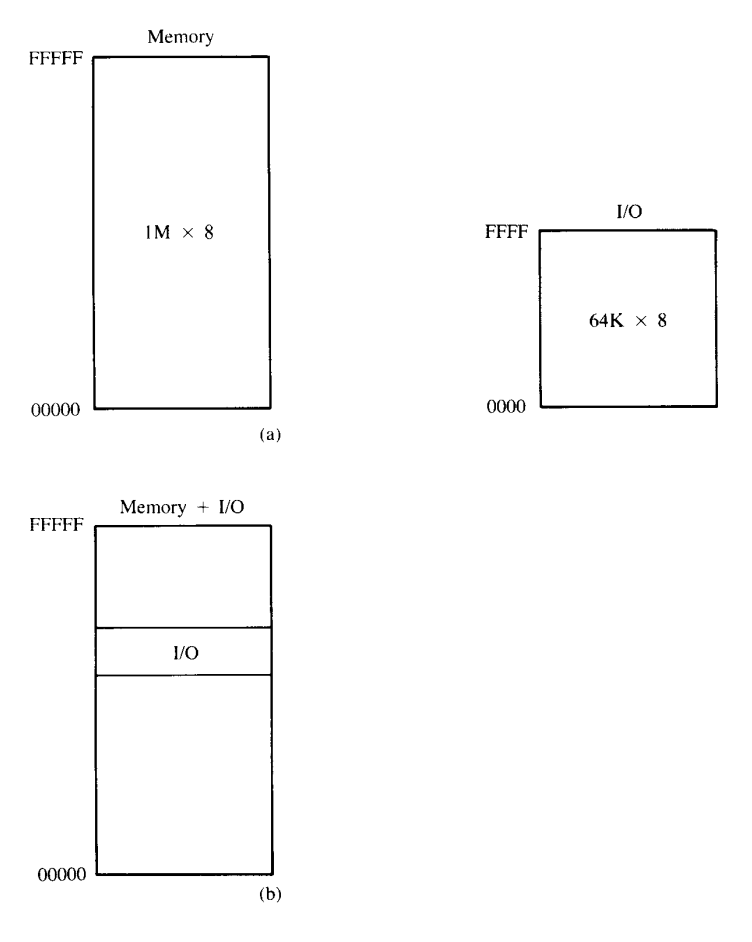
\includegraphics[width = 0.8\textwidth]{./figures/MEM_IO.png}
  \caption{The memory and I/O maps for the 8086/8088 microprocessors.(a) Isolated I/O. (b) Memory-mapped I/O.}
  \label{}
\end{figure}
\textbf{SELF-STUDY}:
\begin{enumerate}
  \item Basic Input Output Interface
  \item I/O port address decoding (Similar as memory)
\end{enumerate}

\section{Programmable Peripheral Interface}
\begin{description}
  \item[82C55]
  \begin{itemize}
    \item low-cost interfacing component having 24 pins for I/O that are programmable in \textit{groups} of 12 pins
    \item It operates in three modes of operations
    \item it is compatible with any TTL-compatible I/O device
    \item Requires insertion of WAIT states in case of operating with a $\mu P$ having more than 8 MHz clock
  \end{itemize}
\end{description}

Basic description of 82C55
\begin{itemize}
  \item Has 3 I/O ports (;abeled as A,B and C)
  \item Programmed as groups
  \begin{enumerate}
    \item Group A: Port A[PA7 - PA0] and upper half of Port C[PC7 - PC4]
    \item Group B: Port B[PB7 - PB0] and lower half of Port C[PC3 - PC0]
  \end{enumerate}
  \item RESET input causes all ports to setup as simple input ports using Mode 0 operation (as setup as input, damage is prevented when power is first applied)
\end{itemize}
\begin{table}[h!]
\centering
\begin{tabular}{ |p{1cm}|p{1cm}|p{3cm}|  }
\hline
$A_1$ & $A_0$ & Function   \\
\hline
0 & 0 & Port A \\
0 & 1 & Port B \\
1 & 0 & Port C \\
1 & 1 & Command Register \\
\hline
\end{tabular}
\caption{Register selection by A1 and A0}
\label{table:11}
\end{table}

\subsection{Programming 2C55: Command Registers}
\begin{figure}[h!]
  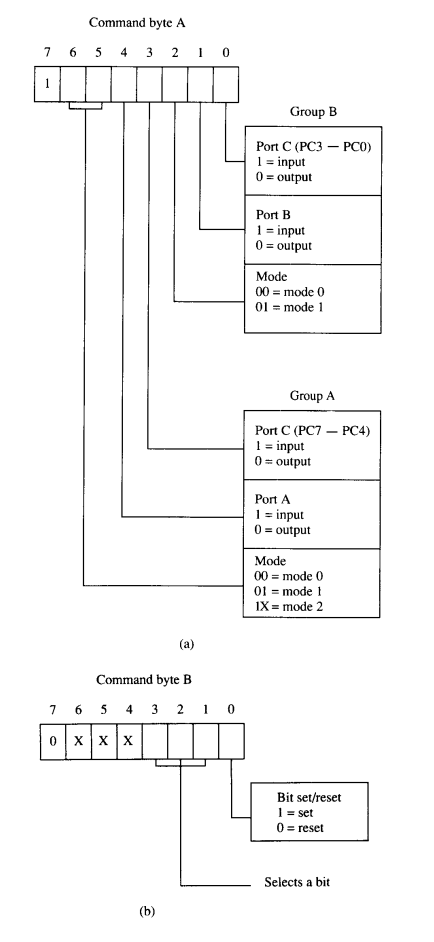
\includegraphics[width = 0.7\textwidth]{./figures/82C55.png}
  \caption{The command byte of the command register in the 82C55. (a) Programs ports A, B, and C. (b) Sets or resets the bit indicated in the select a bit field.}
\end{figure}
\begin{itemize}
  \item
  \textbf{Group A} $\longrightarrow $ 0/1/2 mode \newline
  \textbf{Group B} $\longrightarrow $ 0/1 mode \newline
  \item
  \textbf{Mode 0} $\longrightarrow $ SimpleI/O \newline
  \textbf{Mode 1} $\longrightarrow $ Strobed I/O [Double handshaking I/O] \newline
  \textbf{Mode 2} $\longrightarrow $ Bidirectional Handshaking I/O \newline

\end{itemize}
